\documentclass[tikz,border=2mm]{standalone}
\usepackage{tikz}

\begin{document}
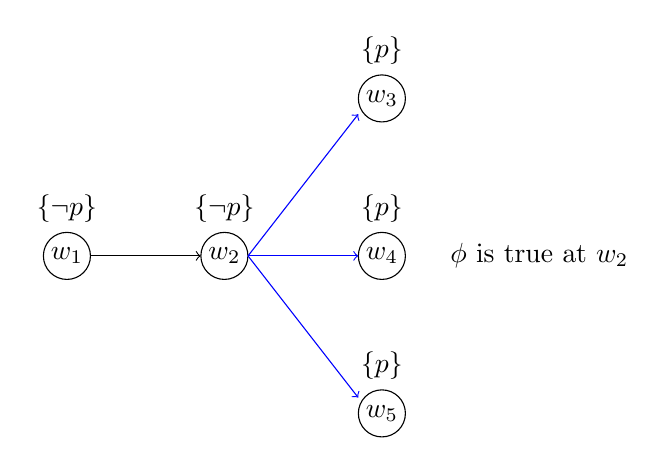
\begin{tikzpicture}[scale=1]
    % Nodes
    \node [label=above:{$\{\neg p\}$}](A) at (0,0) [circle, draw, minimum height=17pt, inner sep=0pt] {$w_1$};
    \node [label=above:{$\{\neg p\}$}](B) at (2,0) [circle, draw, minimum size=17pt, inner sep=0pt] {$w_2$};
    \node [label=above:{$\{ p\}$}](C) at (4,2) [circle, draw, minimum size=17pt, inner sep=1pt] {$w_3$};
    \node [label=above:{$\{ p\}$}](D) at (4,0) [circle, draw, minimum size=17pt, inner sep=1pt] {$w_4$};
    \node [label=above:{$\{ p\}$}](E) at (4,-2) [circle, draw, minimum size=17pt, inner sep=1pt] {$w_5$};

    % Arrows (accessibility relations)
    \draw [->] (0.3,0) -- (1.7,0);
    \draw [->,blue ] (2.3,0) -- (3.7,0);
    \draw [->,blue ] (2.3,0) -- (3.7,1.8);
    \draw [->,blue] (2.3,0) -- (3.7,-1.8);
    \node at (6,0) {$\phi$ is true at $w_2$};
\end{tikzpicture}
\end{document}